\documentclass[11pt, spanish, a4paper, twoside]{article}

% Versión 1.er cuat 2021 Víctor Bettachini < vbettachini@unlam.edu.ar >

\usepackage[T1]{fontenc}
\usepackage[utf8]{inputenc}

\usepackage[spanish, es-tabla]{babel}
% \def\spanishoptions{argentina} % Was macht dass?
% \usepackage{babelbib}
% \selectbiblanguage{spanish}
% \addto\shorthandsspanish{\spanishdeactivate{~<>}}


\usepackage{graphicx}
\graphicspath{{./figuras/}{../LaTeX/}{../figurasLaTeX/}}
% \usepackage{float}

\usepackage[arrowdel]{physics}
\newcommand{\pvec}[1]{\vec{#1}\mkern2mu\vphantom{#1}}
% \usepackage{units}
\usepackage[separate-uncertainty= true, multi-part-units= single, range-units= single, range-phrase= {~a~}, locale= FR]{siunitx}
\usepackage{isotope} % $\isotope[A][Z]{X}\to\isotope[A-4][Z-2]{Y}+\isotope[4][2]{\alpha}

\usepackage{tasks}
\usepackage[inline]{enumitem}
% \usepackage{enumerate}

\usepackage{hyperref}

% \usepackage{amsmath}
% \usepackage{amstext}
% \usepackage{amssymb}

\usepackage{tikz}
\usepackage{tikz-3dplot}
\usepackage{tikz-dimline}
\usetikzlibrary{calc}
% \usetikzlibrary{math}
\usetikzlibrary{arrows.meta}
\usetikzlibrary{snakes}
\usetikzlibrary{decorations}
\usetikzlibrary{decorations.pathmorphing}
\usetikzlibrary{patterns}

\usepackage[hmargin=1cm,vmargin=3cm, top= 0.75cm,nohead]{geometry}

\usepackage{lastpage}
\usepackage{fancyhdr}
\pagestyle{fancyplain}
\fancyhf{}
\setlength\headheight{28.7pt} 
\fancyhead[LE, LO]{\textbf{Mecánica Analítica Computacional} }
% \fancyhead[LE, LO]{\textbf{Mecánica General} }
\fancyhead[RE, RO]{\href{https://ingenieria.unlam.edu.ar/}{$\vcenter{\hbox{
\includegraphics[height=1cm]{ambos.pdf}}}$}}
\fancyfoot{\href{https://creativecommons.org/licenses/by-nc-sa/4.0/deed.es_ES}{$\vcenter{\hbox{
\includegraphics[height=0.4cm]{by-nc-sa_80x15.pdf}}}$} \href{https://ingenieria.unlam.edu.ar/}{DIIT - UNLaM}}
\fancyfoot[C]{ {\tiny Actualizado al \today} }
\fancyfoot[RO, LE]{Pág. \thepage/\pageref{LastPage}}
\renewcommand{\headrulewidth}{0pt}
\renewcommand{\footrulewidth}{0pt}



\begin{document}
\begin{center}
  % \textsc{\large Mecánica general}\\
  \textsc{\large Ligaduras}
\end{center}

\noindent
%De poder resolver estos problemas en forma autónoma puede asumir que adquirió los conocimientos mínimos sobre los temas abordados en la semana.
%No dude en consultar a docentes y compañeros si no puede terminarlos.
Los problemas marcados con (*) tienen alguna dificultad adicional, no dude en consultar.
\begin{enumerate}




%\item \begin{minipage}[t][3.5cm]{0.6\textwidth}
%\textbf{Taylor ej. 7.2}
%Encuentre las ecuaciones de Euler-Lagrange para una partícula moviendose en dos dimensiones usando coordenadas polares.
%Asuma la presencia de una energía potencial \(V(r,\phi)\).
%\end{minipage}
%\begin{minipage}[c][1em][t]{0.35\textwidth}
%	\hspace{0.5cm}
%   \includegraphics[width=0.75\textwidth]{taylorFig7-1}
%\end{minipage}
%


\item 
\begin{minipage}[t][4.5cm]{0.68\textwidth}
	\textbf{Máquina de Atwood simple}\\
	Obtenga a partir de la ecuación de Euler-Lagrange la aceleración que presentan las pesas que cuelgan de una cuerda de longitud \(\ell\) que pasa por sobre una polea de radio \(R\) y masa \(M\).
	\begin{enumerate}
		\item Resuelva el caso en que se considera \(M\) irrelevante.
		\item Resuelva ahora considerando \(M\), y que la polea presenta una sección cilíndrica.
			El momento de inercia de tal cilindro ante rotaciones en torno a su eje de simetría longitudinal es \((M/2) R^2\).
	\end{enumerate}
\end{minipage}
\begin{minipage}[c][0cm][t]{0.3\textwidth}
	% \hspace{0.5cm}
	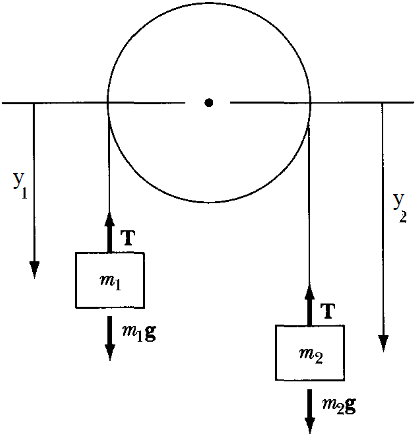
\includegraphics[width=0.75\textwidth]{marion_fig2_11a}
	% 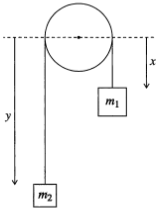
\includegraphics[width=0.75\textwidth]{marion_fig2_1a}
\end{minipage}


\item 
\begin{minipage}[t][5cm]{0.75\textwidth}
\textbf{Aro y polea}\\
	Una partícula de masa \(M\) se está ligada a un aro de radio \(R\) y masa despreciable dispuesto verticalmente que rota libremente en torno a su centro fijo.
	La partícula está atada por una cuerda que se enrolla parcialmente en torno al aro, luego asciende verticalmente y pasa por una polea de masa \(m_p\).
	Otra partícula de masa \(m < M\) pende del otro extremo de la cuerda de longitud \(\ell\).
	El aro de masa \(m_a\) tiene un momento de inercia para rotaciones en torno a su eje de simetría longitudinal de \(m R^2\).
	\begin{enumerate}
		\item (*) Describa la ligadura contemplando el ángulo de rotación del aro.
		\item Obtenga la ecuación de Euler-Lagrange para la dinámica.
\end{enumerate}
\end{minipage}
\begin{minipage}[c][0cm][t]{0.2\textwidth}
	% \hspace{0.5cm}
	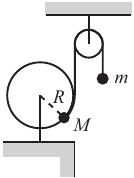
\includegraphics[width=0.75\textwidth]{cmchap6_fig6_14}
\end{minipage}


\item 
\begin{minipage}[t][5.5cm]{0.7\textwidth}
	\textbf{Péndulo de pesas engarzadas y acopladas}\\ 
	Dos partículas de masa \(m_1\) y \(m_2\) están unidas por una barra rígida inextensible de longitud \(\ell\) y masa despreciable frente a las anteriores.
	La de \(m_1\) se mueve solo sobre el eje \(x\) y la de \(m_2\) solo sobre el \(y\).
\begin{enumerate}
	\item Despeje la aceleración en la ecuación de Euler-Lagrange para una única coordenada generalizada\\
	\begin{enumerate*}[
				itemjoin=\quad,
				before=\hspace*{\fill},
				after=\hspace*{\labelwidth}\hspace*{-\labelsep}\hspace*{\fill},
			]
		\item \(y\)
		\item \(\theta\)
	\end{enumerate*}\\ % https://tex.stackexchange.com/questions/591120/how-can-you-put-items-on-one-line-and-center-them
	Tras resolver ambos casos, ¿cuál preferiría para trabajar?
	\item (*) ¿Cuál es el período de movimiento de pequeñas oscilaciones para el caso \(m_1 = m_2 = m\)?
\end{enumerate}
\end{minipage}
\begin{minipage}[c][0cm][t]{0.3\textwidth}
	% \hspace{0.5cm}
	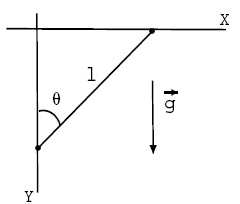
\includegraphics[width=0.75\textwidth]{fcen1-004}
\end{minipage}



\item
\begin{minipage}[t][6cm]{0.6\textwidth}
\textbf{Maquina de Atwood compuesta} [Marion (english) ex. 7.8]\\ 
\begin{enumerate}
	\item Obtenga las aceleraciones en este sistema resolviendo las ecuaciones de Euler-Lagrange.
	Las coordenadas se reducen a dos, \(x\) e \(y\), pues con el vínculo de las cuerdas establece la posición de todas las masas y de la polea inferior.
	Simplifique el problema considerando que las poleas de radio \(R\) tienen masa nula (\(M=0\)).
	\item (*) Contemple ahora la masa de las poleas \(m_p\).
	Recuerde que el momento de inercia de un cilindro es \((m/2) R^2\)
\end{enumerate}
\end{minipage}
\begin{minipage}[c][0.5em][t]{0.3\textwidth}
%		\begin{tikzpicture}
%			\draw [ultra thick] (-2,4) -- (2,4);
%			\fill [pattern = north east lines] (-2,4) rectangle (2,4.2); % techo
%			\draw (0,4) -- (0,3); % linea vertical techo - polea superior
%			\draw (0,3) circle [radius=0.5]; % polea superior
%			\draw (-0.5,3) -- (-0.5,1.5); % linea vertical izquierda polea sup - inf
%			\draw (0.5,3) -- (0.5,2.25); % linea vertical izquierda polea sup - m3
%			\draw (0.25,1.75) rectangle (0.75,2.25) node [anchor= north west] {\(m_3\)} ; % m3
%			% \draw (0.25,1.75) node [above=1, right=9.6] {\(m_3\)} rectangle (0.75,2.25) node [above=1, right=9.6] {\(m_3\)} ; % m3
%			\draw (-0.5,1.5) circle [radius=0.5]; % polea inferior
%			\draw (-1,1.5) -- (-1,.25); % linea vertical izquierda polea inf - m1
%			\draw (-1.25,-.25) rectangle (-0.75,0.25) node [anchor= north west] {\(m_1\)} ; % m1
%			\draw (0,1.5) -- (0,1); % linea vertical izquierda polea inf - m2
%			\draw (-.25,.5) rectangle (.25,1) node [anchor= north west] {\(m_2\)} ; % m2
%		\end{tikzpicture}
	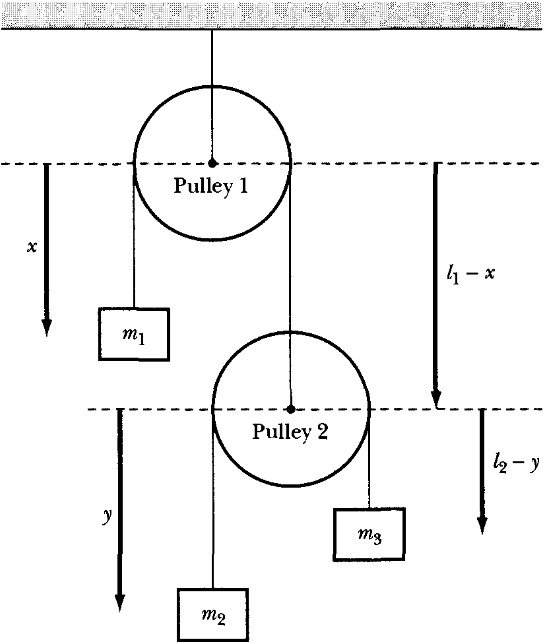
\includegraphics[width=\textwidth]{marion_fig7_6}
\end{minipage}




\end{enumerate}
\end{document}
